\documentclass{article}
\usepackage[utf8]{inputenc}
\usepackage{listings}
\usepackage{multimedia} % to embed movies in the PDF file
\usepackage{graphicx}
\usepackage{comment}
\usepackage[english]{babel}
\usepackage{amsmath}
\usepackage{amsfonts}
\usepackage{subfigure}
\usepackage{wrapfig}
\usepackage{multirow}
\usepackage{tikz}
\usepackage{verbatim}

\newtheorem{theorem}{Theorem}[section]
\newtheorem{lemma}[theorem]{Lemma}
\newtheorem{corollary}[theorem]{Corollary}
%\newtheorem{algorithm}[theorem]{Algorithm}
\newtheorem{remark}[theorem]{Remark}
\newenvironment{proof}{\noindent {\bf Proof:} }{\hfill $\Box$ \\[2ex] }
\newenvironment{keywords}{\begin{quote} {\bf Key words} }
                         {\end{quote} }
\newenvironment{AMS}{\begin{quote} {\bf AMS subject classifications} }
                         {\end{quote} }


\newcommand{\eref}[1]{\mbox{\rm(\ref{#1})}}
\newcommand{\tref}[1]{\mbox{\rm\ref{#1}}}
\newcommand{\set}[2]{\left\{ #1 \; : \; #2 \right\} }
\newcommand{\deq}{\raisebox{0pt}[1ex][0pt]{$\stackrel{\scriptscriptstyle{\rm def}}{{}={}}$}}

\newcommand {\DS} {\displaystyle}

\newcommand{\real}{\mathbb{R}}
\newcommand{\compl}{\mathbb{C}}



\newcommand {\half} {\mbox{$\frac{1}{2}$}}
\newcommand{\force}{{\mathbf{f}}}
\newcommand{\strain}{{\boldsymbol{\varepsilon}}}
\newcommand{\stress}{{\boldsymbol{\sigma}}}
\renewcommand{\div}{{\boldsymbol{\nabla}}}

\newcommand {\cA} {{\cal A}}
\newcommand {\cB} {{\cal B}}
\newcommand {\cC} {{\cal C}}
\newcommand {\cD} {{\cal D}}
\newcommand {\cE} {{\cal E}}
\newcommand {\cL} {{\cal L}}
\newcommand {\cP} {{\cal P}}
\newcommand {\cQ} {{\cal Q}}
\newcommand {\cR} {{\cal R}}
\newcommand {\cV} {{\cal V}}
\newcommand {\cW} {{\cal W}}
\newcommand {\CH} {{\cal H}}
\newcommand {\CS} {{\cal S}}


\newcommand{\bzero}{\mathbf{0}}
\newcommand{\ba}{\mathbf{a}}
\newcommand{\bb}{\mathbf{b}}
\newcommand{\bc}{\mathbf{c}}
\newcommand{\bd}{\mathbf{d}}
\newcommand{\be}{\mathbf{e}}
\newcommand{\bff}{\mathbf{f}}
\newcommand{\bg}{\mathbf{g}}
\newcommand{\bh}{\mathbf{h}}
\newcommand{\bn}{\mathbf{n}}
\newcommand{\bp}{\mathbf{p}}
\newcommand{\bq}{\mathbf{q}}
\newcommand{\br}{\mathbf{r}}
\newcommand{\bs}{\mathbf{s}}
\newcommand{\bt}{\mathbf{t}}
\newcommand{\bu}{\mathbf{u}}
\newcommand{\bv}{\mathbf{v}}
\newcommand{\bw}{\mathbf{w}}
\newcommand{\bx}{\mathbf{x}}
\newcommand{\by}{\mathbf{y}}
\newcommand{\bz}{\mathbf{z}}
\newcommand{\bA}{\mathbf{A}}
\newcommand{\bB}{\mathbf{B}}
\newcommand{\bC}{\mathbf{C}}
\newcommand{\bD}{\mathbf{D}}
\newcommand{\bE}{\mathbf{E}}
\newcommand{\bF}{\mathbf{F}}
\newcommand{\bG}{\mathbf{G}}
\newcommand{\bH}{\mathbf{H}}
\newcommand{\bI}{\mathbf{I}}
\newcommand{\bJ}{\mathbf{J}}
\newcommand{\bK}{\mathbf{K}}
\newcommand{\bL}{\mathbf{L}}
\newcommand{\bM}{\mathbf{M}}
\newcommand{\bN}{\mathbf{N}}
\newcommand{\bO}{\mathbf{O}}
\newcommand{\bP}{\mathbf{P}}
\newcommand{\bQ}{\mathbf{Q}}
\newcommand{\bR}{\mathbf{R}}
\newcommand{\bS}{\mathbf{S}}
\newcommand{\bU}{\mathbf{U}}
\newcommand{\bV}{\mathbf{V}}
\newcommand{\bW}{\mathbf{W}}
\newcommand{\bX}{\mathbf{X}}
\newcommand{\bY}{\mathbf{Y}}
\newcommand{\bZ}{\mathbf{Z}}

\newcommand{\cO}{ {\cal O} }
\newcommand{\CT}{ {\cal T} }
\newcommand{\IL}{{\mathbb L}}
\newcommand{\sIL}{{{{\mathbb L}_s}}}
\newcommand{\bOmega}{{\boldsymbol{\Omega}}}
\newcommand{\bPsi}{{\boldsymbol{\Psi}}}

\newcommand{\bgamma}{{\boldsymbol{\gamma}}}
\newcommand{\bmu}{{\boldsymbol{\mu}}}
\newcommand{\blambda}{{\boldsymbol{\lambda}}}
\newcommand{\bLambda}{{\boldsymbol{\Lambda}}}
\newcommand{\bpi}{{\boldsymbol{\pi}}}
\newcommand{\bPi}{{\boldsymbol{\Pi}}}
\newcommand{\bphi}{{\boldsymbol{\phi}}}
\newcommand{\bPhi}{{\boldsymbol{\Phi}}}
\newcommand{\bpsi}{{\boldsymbol{\psi}}}
\newcommand{\btheta}{{\boldsymbol{\theta}}}
\newcommand{\bTheta}{{\boldsymbol{\Theta}}}
\newcommand{\bSigma}{{\boldsymbol{\Sigma}}}
\newcommand{\sump}{\sideset{}{^{'}}\sum} 
\DeclareMathOperator*{\Res}{Res}
\DeclareMathOperator{\OO}{O}
\DeclareMathOperator{\oo}{o}
\DeclareMathOperator{\erfc}{erfc}
\def\Xint#1{\mathchoice
   {\XXint\displaystyle\textstyle{#1}}%
   {\XXint\textstyle\scriptstyle{#1}}%
   {\XXint\scriptstyle\scriptscriptstyle{#1}}%
   {\XXint\scriptscriptstyle\scriptscriptstyle{#1}}%
   \!\int}
\def\XXint#1#2#3{{\setbox0=\hbox{$#1{#2#3}{\int}$}
     \vcenter{\hbox{$#2#3$}}\kern-.5\wd0}}
\def\ddashint{\Xint=}
\def\pvint{\Xint-}





\title{AMATH 570 Assignment 4}
\author{Cade Ballew}
\date{November 10, 2021}

\begin{document}

\maketitle

\section{Problem 1}
\subsection{Exercise 10.4}
Let $f\in C([-1, 1])$ be an
even function for all $x$.
\subsubsection{Part a}
To show that for any $n\in\mathbb{N}$, the best approximation $p_n^*$ is even, we consider an approximation $e(x)$ that is even and show that we cannot improve it by adding an odd function $o(x)$. To see this, first observe that 
\begin{align*}
||f-e||_\infty&=\max_{x\in[-1,1]}|f(x)-e(x)|=\max\left\{\max_{x\in[-1,0)}|f(x)-e(x)|,\max_{x\in[0,1]}|f(x)-e(x)|\right\}\\&=
\max\left\{\max_{x\in(0,1]}|f(-x)-e(-x)|,\max_{x\in[0,1]}|f(x)-e(x)|\right\}\\&=\max\left\{\max_{x\in(0,1]}|f(x)-e(x)|,\max_{x\in[0,1]}|f(x)-e(x)|\right\}\\&=
\max_{x\in[0,1]}|f(x)-e(x)|
\end{align*}
Similarly, 
\begin{align*}
||f-(e+o)||_\infty&=\max_{x\in[-1,1]}|f(x)-e(x)-o(x)|\\&=
\max\left\{\max_{x\in[-1,0)}|f(x)-e(x)-o(x)|,\max_{x\in[0,1]}|f(x)-e(x)-o(x)|\right\}\\&=
\max\left\{\max_{x\in(0,1]}|f(-x)-e(-x)-o(-x)|,\max_{x\in[0,1]}|f(x)-e(x)-o(x)|\right\}\\&=\max\left\{\max_{x\in(0,1]}|f(x)-e(x)+o(x)|,\max_{x\in[0,1]}|f(x)-e(x)-o(x)|\right\}.
\end{align*}
It is clear that $||f-(e-o)||_\infty\leq||f-e||_\infty$ only if $o(x)=0$ because we $o(x)$ is both added and subtracted and we take the maximum of the two. Thus, an even approximation $e(x)$ can only be improved by adding another even function, meaning that the best approximation is even. 

\subsubsection{Part b}
From part $a$, we know that $p_{2n+1}^*$ must be an even function for $n\in\mathbb{N}$. However, this means that the coefficient on $x^{2n+1}$ in $p_{2n+1}^*$ must be 0, meaning that $p_{2n+1}^*\in\mathcal{P}_n$. By definition $p_{2n}^*$ is the best approximation in ${P}_n$, so it must hold that $p_{2n+1}^*=p_{2n}^*$.
\subsubsection{Part c}
Now, say that $f\in C([-1, 1])$ is not even. For sufficiently large $n$, its best approximation $p_n^*$ is also not even. This is because our sequence of best approximations should converge to $f$ which is not even, so for sufficiently large $n$, our best approximation should be even in order to not have a large error at some point. Otherwise, our sequence would fail to converge to $f$ and fail to be the best approximation as a result.   

\subsection{Exercise 10.6}
To see that the operator that maps a function $f\in C([-1, 1])$ to its best degree n
approximation $p_n^*$ is nonlinear, consider $f_1(x)=x$, $f_2(x)=|x|$, and $n=0$. Then, the best approximation to $f_1$ is $p_0^*=0$ and the best approximation to $f_2$ is $p_0^*=1/2$. However,  the best approximation to $f_1+f_2$ is $p_0^*=1$ which is not the sum of the best approximations.

\subsection{Exercise 10.12}
Let $p$ be the best approximation in $\mathcal{P}_n$ to a real function $f\in C([-1, 1])$. We know that $f-p$ has $n+2$ equioscillations of opposite signs and is also continuous because both $p$ and $f$ are continuous. Thus, $f-p$ must have a zero between any two consecutive equiosciallation points by the intermediate value theorem. There are $n+2$ of these, so $f-p$ has at least $n+1$ zeroes, meaning that $p$ interpolates $f$ at $n+1$ (but not more due to $p$ having degree $n$) points (which of course are distinct). 

\subsection{Exercise 11.1}
\subsubsection{Part a}
To find the polynomial $p\in\mathcal{P}_n$ that takes values $p(-1) = 1$, $p(1/2) = 2$, and $p(1) = 2$, let $p(x)=ax^2+bx+c$ and plug these values in to get the system
\begin{align*}
a-b+c=1\\
\frac{a}{4}+\frac{b}{2}+c=2\\
a+b+c=2.
\end{align*}
Subtracting the first and third equations, we quickly get that $-2b=-1$, so $b=1/2$. Then, we can reduce the system to
\begin{align*}
a+4c=7\\
a+c=\frac{3}{2}.
\end{align*}
Subtracting, we get $3c=11/2$, so $c=11/6$. This implies that $a=-1/3$. Thus,
\[
p(x)=-\frac{1}{3}x^2+\frac{1}{2}x+\frac{11}{6}
\]
and $p(2)=-4/3+1+11/6=3/2$.
\subsubsection{Part b}
We verify the Hermite integral formula for p(2) and $f(x)=(x+1)(x-0.5)(x-1)e^x+ 11/6+x/2-x^2/3$ via chebfun for contours $|x|=3/2$ and $|x|=3$. As expected, both give that the integral evaluates to 1.5. See problem11\_1.m for the code that does this.

\subsubsection{Part c}
Making this evaluation into a anonymous function and taking the chebfun of this function, the command poly gives that the coefficients are 
\begin{verbatim}
-0.3333 + 0.0000i   0.5000 + 0.0000i   1.8333 - 0.0000i
\end{verbatim}
which match the coefficients we found in part a. See problem11\_.m for the code that does this. 

\section{Problem 2} 
We wish to show that our two definitions of the $\epsilon$-pseudospectrum
\begin{enumerate}
\item 
\[
\Lambda_{\epsilon} (A) = \{ z \in \mathbb{C} : z \mbox{ is an eigenvalue of $A+E$
for some $E$ with $\| E \| < \epsilon$} \} .
\]
\item
\[
\Lambda_{\epsilon} (A) = \{ z \in \mathbb{C} : \| (zI - A )^{-1} \| > \epsilon^{-1} \} .
\]
\end{enumerate}
are equivalent. First, let $z$ be an eigenvalue for some $E$ with $\| E \| < \epsilon$. Then, by definition there must be some eigenvector $v$ such that $(A+E)v=zv$ and $\|v\|=1$. Thus, $(zI-A)v=Ev$ and $v=(zI-A)^{-1}Ev$. Then,
\begin{align*}
1&=\|v\|=\|(zI-A)^{-1}Ev\|\leq\|(zI-A)^{-1}E\|\|v\|\\&\leq\|(zI-A)^{-1}\|\|E\|<||(zI-A)^{-1}||\epsilon.
\end{align*}
Thus, $\|(zI - A )^{-1} \| > \epsilon^{-1}$. \\
Now, let $z\in\mathbb{C}$ be such that $\|(zI - A )^{-1} \| > \epsilon^{-1}$. Then, by definition, there exists some vector $v$ such that $\|v\|=1$ and $\|(zI - A )^{-1} v\| > \epsilon^{-1}$. Define $w=(zI - A )^{-1} v$. Then, $(zI - A )v=w$, so $(zI - A -\frac{vw^*}{w^*w})w=0$ (note that $w^*w\neq0$), and $(A +\frac{vw^*}{w^*w})w=zw$. Thus, if we take $E=\frac{vw^*}{w^*w}$, then $z$ is an eigenvalue of $A+E$. Also,
\begin{align*}
\|E\|^2&=\|EE^*\|=\|\frac{vw^*}{w^*w}\frac{wv^*}{w^*w}\|=\|\frac{v(w^*w)v^*}{(w^*w)^2}\|\leq\|\frac{vv^*}{w^*w}\|\leq\|v\|\|v^*\|\left|\frac{1}{w^*w}\right|\\&=
\frac{1}{\|w\|^2}<\epsilon^2
\end{align*}
because $w^*w$ is a projection matrix is a scalar and $\|v\|=1$. Thus, $\|E\|<\epsilon$.

\section{Problem 3}
\subsection{Exercise 10.3}
Solving the initial boundary value problem in MATLAB as requested, we get the following plots when $\nu=7$:\\
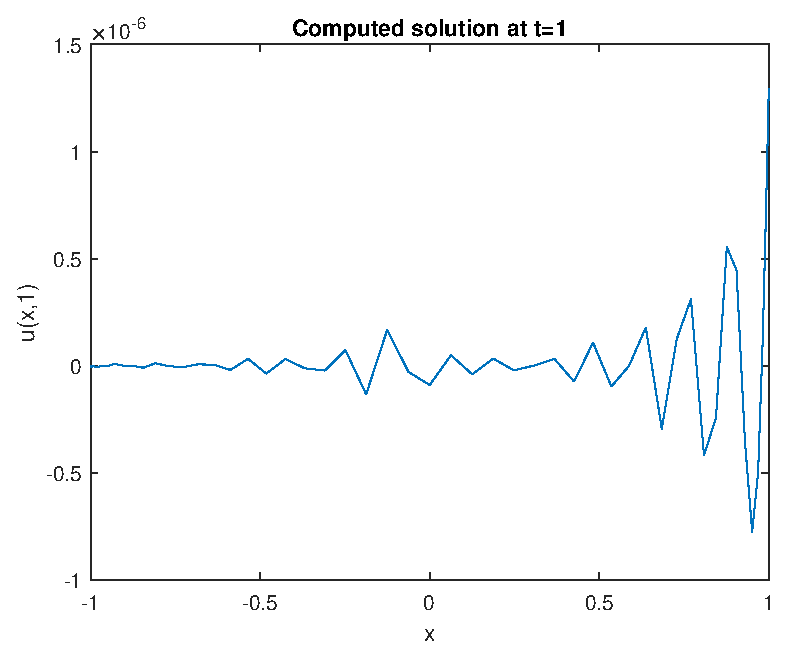
\includegraphics[scale=0.8]{sol7.eps}\\
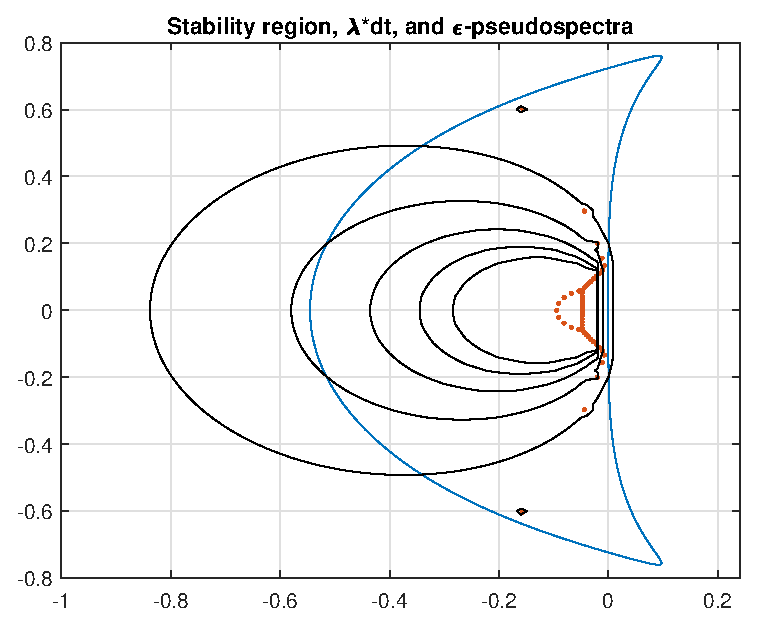
\includegraphics[scale=0.8]{reg7.eps}\\
\\
If we instead take $\nu=8$, we get \\
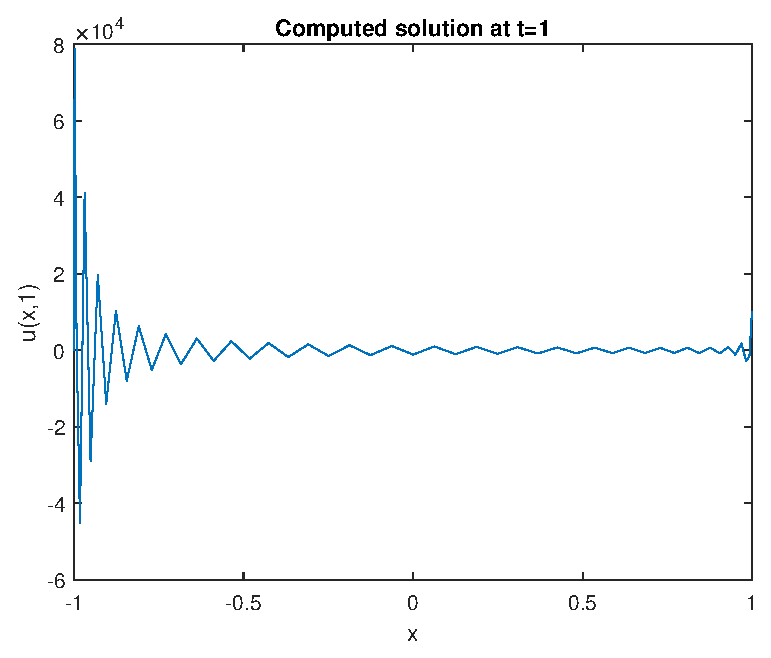
\includegraphics[scale=0.8]{sol8.eps}\\
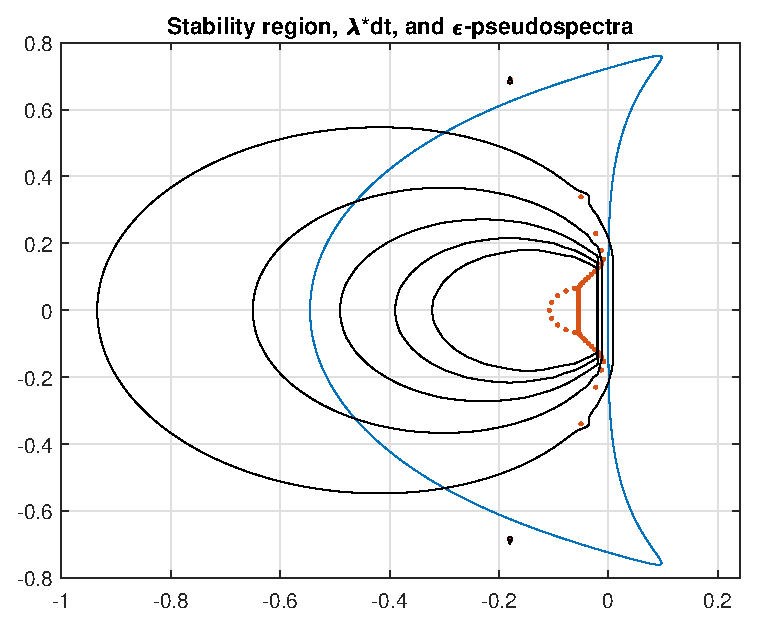
\includegraphics[scale=0.8]{reg8.eps}\\
Clearly, the scheme is stable in the first case but not in the second. We can see why from the stability region as all eigenvalues are inside the region in the first case but not in the second which leads to the solution "blowing up" when we take $\nu=8$. \\
See problem10\_3.m for the code that does this.

\subsection{Exercise 10.4}
To approximate the solution of the nonlinear initial boundary value problem, we take a small spatial grid $N=16$ and a very small timestep to ensure stability and use the Chebyshev differentiation matrix in space and an RK4 discretization in time. From this, we approximate that $u(0,3.5)=3.5389363$. We also find that $u(0,t_5)=5$ at approximately $t_5=3.535936$ very soon after. \\
See problem10\_4.m for the code that does this.

\end{document}
